% !TeX root = ../notes.tex

\section{Social Linked Data}

\begin{itemize}
    \item Data Space Konzept basierend auf \emph{Semantic Web} und \emph{Social Linked Data} (Solid)
    \item Fundament für offene, dezentralisierte Netzwerke für souveränen Datenaustausch~\cite{mecklerWebLinkedData2023}
\end{itemize}

\vspace{1cm}

\textbf{Solid}
\begin{itemize}
    \item Bewegung zur Garantie von Datensouveränität~\cite{mecklerWebLinkedData2023}
    \item definiert Protokolle zur Verwaltung von persönlichen Daten in einer dezentralisierten Umgebung basierend auf W3C"=Empfehlungen~\cite{mecklerWebLinkedData2023}
    \item Speicherung von (un)strukturierten Daten in \emph{Personal Online Data Stores} (Pods)~\cite{mecklerWebLinkedData2023}
\end{itemize}


\subsection{Solid Data Spaces}

\begin{itemize}
    \item Verwendung der Web"=Architektur und Solid als Fundament für DS
    \item Erweiterung von Web"=Technologien und "=Frameworks für Schaffung einer Umgebung für sicheren Datenaustausch~\cite{mecklerWebLinkedData2023}
\end{itemize}

\subsubsection{Technologie-Schichten in SDS}

\begin{itemize}
    \item Web Layer: interoperable Kommunikation und Plattformunabhängigkeit
    \begin{itemize}
        \item einheitliche Komm. via HTTP(S)
        \item Sicherheit durch Verschlüsselung via TLS
        \item bekannte Datenformate: XML, JSON, HTML
    \end{itemize}
    
    \item Linked Data: Repräsentation der Daten mittels RDF und \emph{Shared Vocabularies}
    \begin{itemize}
        \item Menschen- und Maschinen-verständlich
    \end{itemize}

    \item Solid: Access"=Layer
    \begin{itemize}
        \item Vereinbarung zur Verwaltung von Daten, Identitäten und Zugriffskontrolle
    \end{itemize}

    \item Data Space als Application"=Layer
    \begin{itemize}
        \item Anwendungs"=Interoperabilität
        \item zusätzliche, anwendungsspezifische Vereinbarung
        \item DS-Authorities: Überwachung des Data Sharing Prozesses~\cite{mecklerWebLinkedData2023}
    \end{itemize}
\end{itemize}

\vspace{1cm}

\begin{itemize}
    \item Schritt-für-Schritt Einführung möglich
    \item geringe Einstiegsbarriere~\cite{mecklerWebLinkedData2023}
\end{itemize}


\subsubsection{Hauptkomponenten in SDS}

\begin{figure}
    \centering
    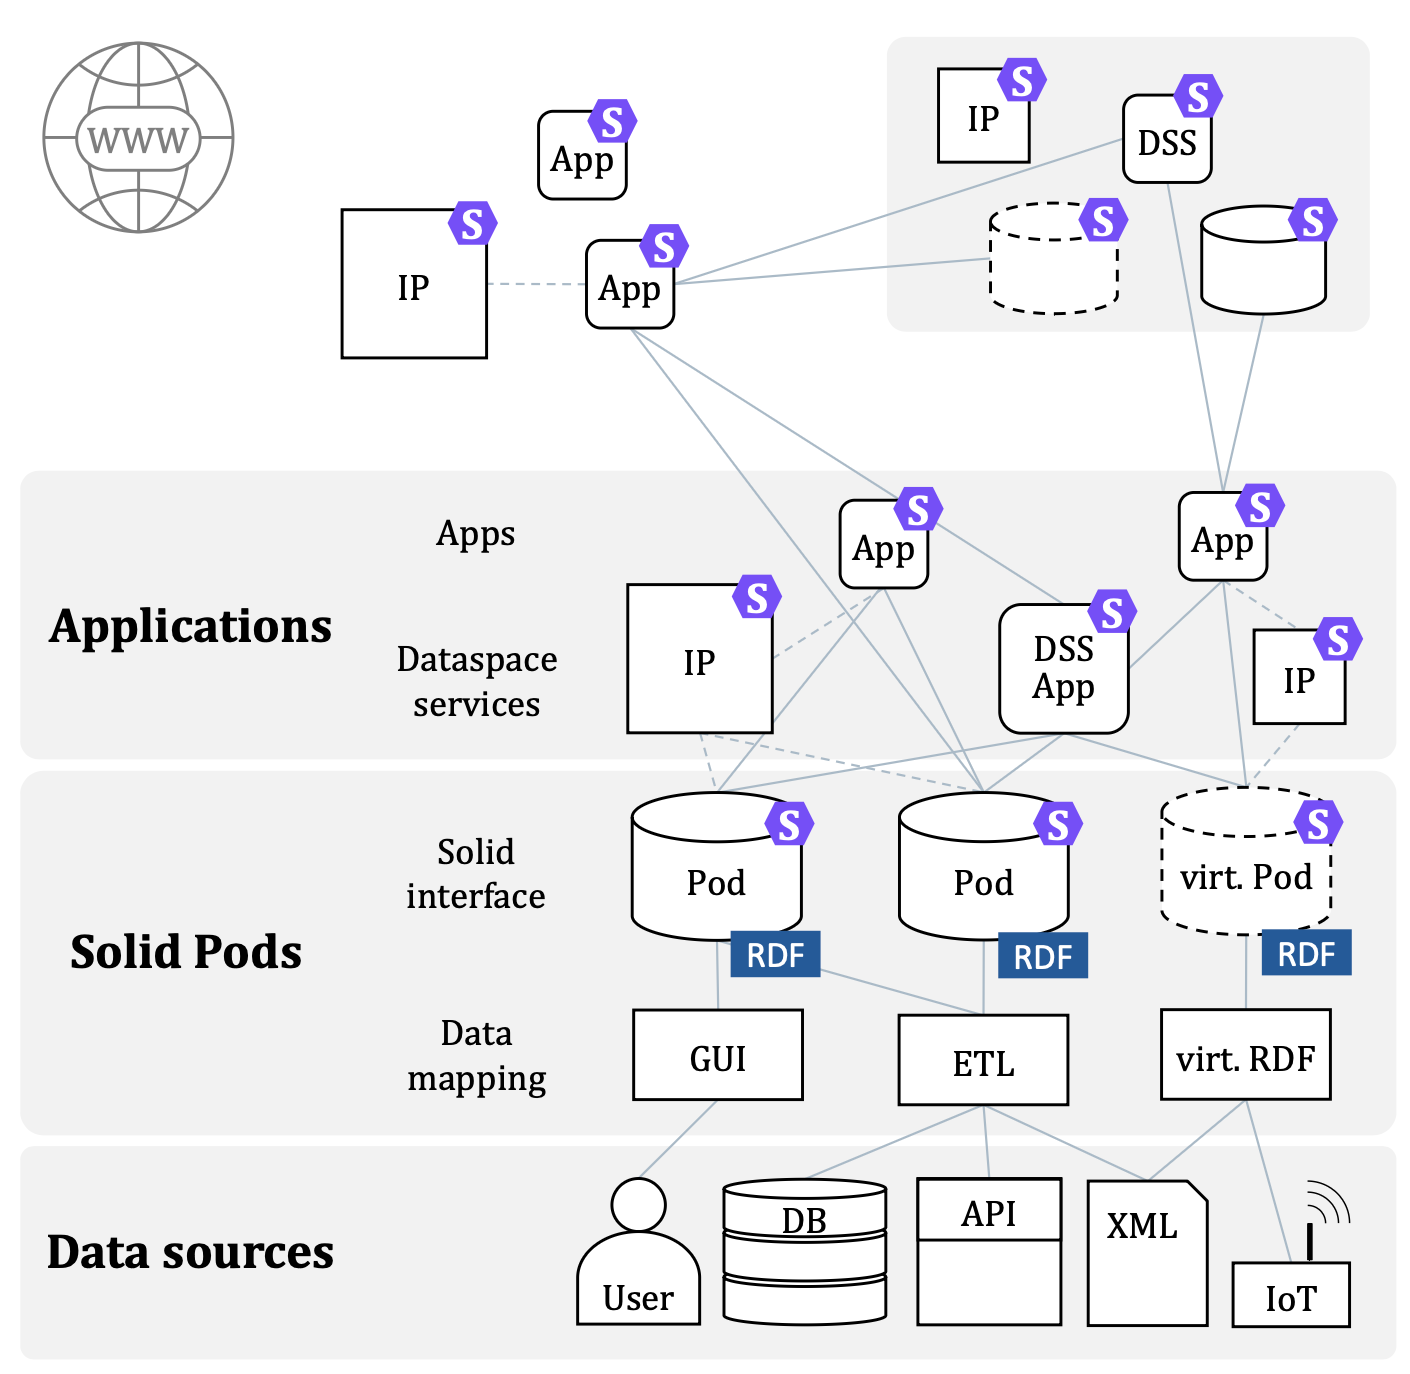
\includegraphics[width=0.7\textwidth]{../shared/assets/meckler_sds_components.png}
    \caption{Komponenten eines Solid Data Spaces~\cite{mecklerWebLinkedData2023}}
\end{figure}

\begin{itemize}
    \item Identity Provider (IdP)
    \begin{itemize}
        \item IdP eines Unternehmens verifizieren Identität eines Akteurs
    \end{itemize}
    
    \item Solid Server
    \begin{itemize}
        \item Hosten mehrerer Pods
        \item Pods: Datenspeicherung und Zugriffsregeln
    \end{itemize}
    
    \item Solid Anwendungen
    \begin{itemize}
        \item allg. Web-Apps, welche Operationen auf Solid Pods ausführen
        \item Bereitstellung von DS-Service oder andere Zwecke
        \item DS-Service-Apps (DSS Apps)
        \begin{itemize}
            \item \enquote{discovery, search and query, monitoring, or administration}~\cite{mecklerWebLinkedData2023}
            \item Vereinbarungen zwischen Teilnehmern eines DS zum Anbieten von Services (vgl. App Store)
        \end{itemize}
    \end{itemize}

    \item Data Mapping von verschiedenen Standards zu RDF
    \begin{itemize}
        \item lesbar für Mensch und Maschine (automatisierbar)
        \item Referenzierung von Klassen und Properties aus Ontologien
        \item Verwendung von Shared Vocabularies, Implementierung von \hl{Linked Data Prinzipien} $\Rightarrow$ selbsterklärende Daten, vernetzt mit verwandten Ressourcen
    \end{itemize}

    \item Integration von RDF-Daten via \emph{Extract-Transform-Load} (ETL) oder via GUI
    \item binäre Daten in Pods zusammen mit Metadaten~\cite{mecklerWebLinkedData2023}
\end{itemize}

% TODO: Vgl. SDS IDS (@mecklerWebLinkedData2023)


\subsection{Identität und Authentifizierung}

\begin{itemize}
    \item Authentifizierungsprotokolle
    \begin{itemize}
        \item Ermittlung der Identität und Profildaten
        \item Ermittlung relevanter Links zum Pod und Anwendungsdaten~\cite{sambraSolidPlatformDecentralized2016}
    \end{itemize}
    \item dezentralisierte Auth., globaler ID"=Space \& globales SSO als Fundament von Solid Ökosystemen $\to$ WebID~\cite{sambraSolidPlatformDecentralized2016}
    \begin{itemize}
        \item WebID da gut zu RDF"=basierten Profildaten und Erweiterbarkeit passend~\cite{sambraSolidPlatformDecentralized2016}
    \end{itemize}

    \item Registrierung über Identity Provider, meist bei Pod"=Provider~\cite{sambraSolidPlatformDecentralized2016}
    \begin{itemize}
        \item Speicherung des \emph{Web ID Profile Document} sowie kryptografischer Schlüssel
    \end{itemize}
\end{itemize}

\begin{figure}
    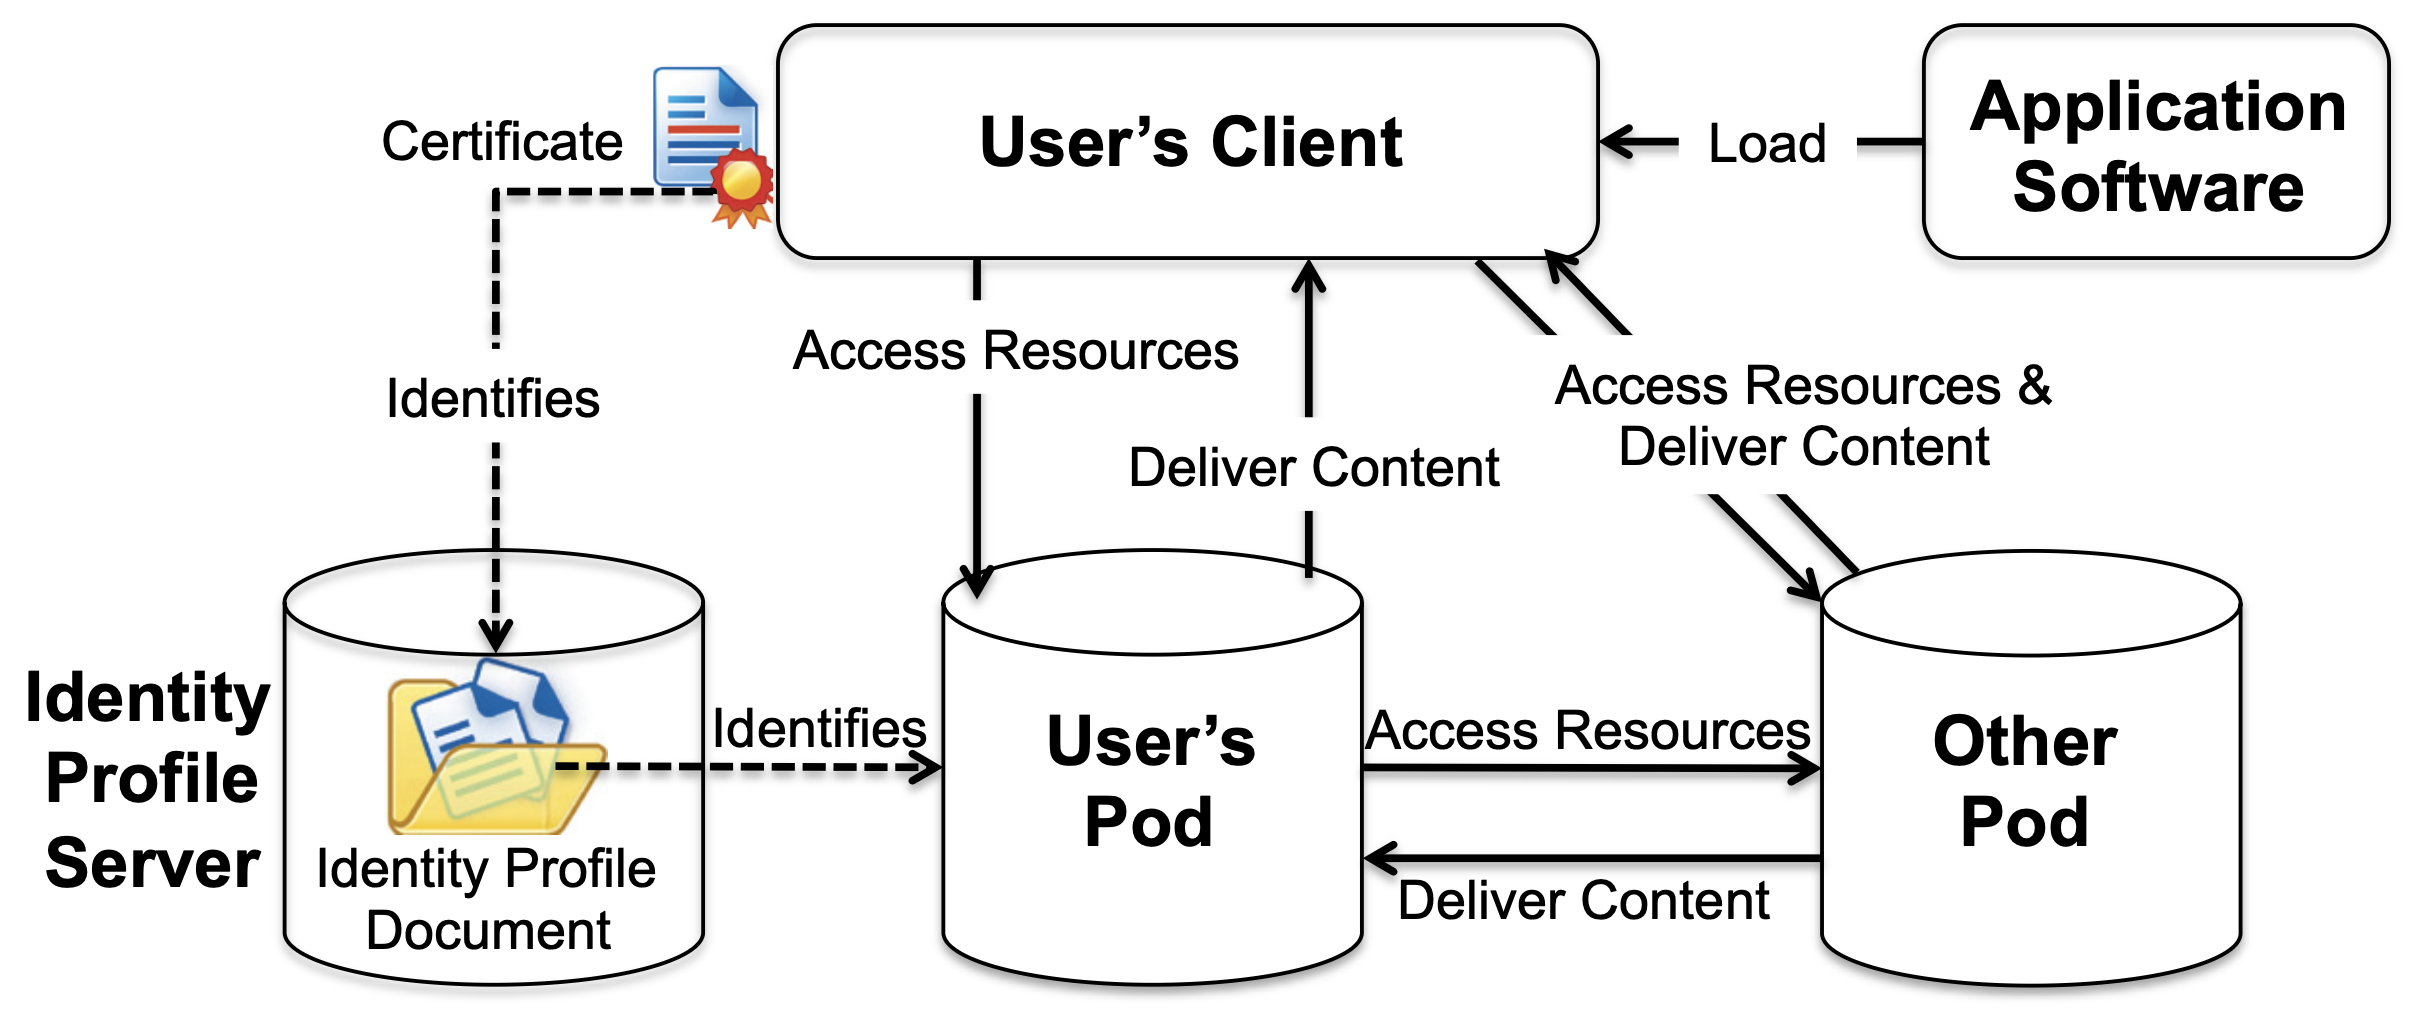
\includegraphics[width=\textwidth]{../shared/assets/sambra_solid_architecture.png}
    \caption{Solid Architektur~\cite{sambraSolidPlatformDecentralized2016}}
\end{figure}

\vspace{1cm}

\textbf{Dezentralisierte Identität basierend auf WebID}
\begin{itemize}
    \item für tatsächliche Dezentralisierung ist globaler \emph{Identity Space} notwendig~\cite{sambraSolidPlatformDecentralized2016}
    \item WebID für globales Identitätsmanagement basierend auf System dezentralisierter IdPs~\cite{sambraSolidPlatformDecentralized2016}
    \item jede Person muss eigene Identität kontrollieren können, Identität muss über mehrere Seiten hinweg verlinkbar sein $\to$ \emph{Web of Relations}~\cite{sambraSolidPlatformDecentralized2016}
    \item \emph{Agenten} (Personen, Unternehmen oder andere Gruppen) erstellen eigene Identität durch Verlinkung einer HTTP(S)-URI mit einem \emph{Profile Document}~\cite{sambraSolidPlatformDecentralized2016}
    \begin{itemize}
        \item PDoc: Webseite im RDF"=Format~\cite{sambraSolidPlatformDecentralized2016}
        \item URI global eindeutig~\cite{mecklerWebLinkedData2023}
        \item enthält alle notwendigen Informationen, um \emph{Web of Trust} zu erzeugen durch Verlinkung von Profilen miteinander~\cite{sambraSolidPlatformDecentralized2016}
    \end{itemize}
    \item Web of Trust $\to$ Auth.-Entscheidungen basierend auf Eigenschaften von Agenten (bspw. Beziehung zu anderen Agenten, Arbeitsstelle etc.)~\cite{sambraSolidPlatformDecentralized2016}
\end{itemize}

\vspace{1cm}

\textbf{WebID-TLS Authentifizierung}
\begin{itemize}
    \item dezentralisiertes Auth."=Protokoll~\cite{sambraSolidPlatformDecentralized2016}
    \item Authentifizierung~\cite{sambraSolidPlatformDecentralized2016}
    \begin{itemize}
        \item Nutzer:in möchte sich auth.
        \item Browser schlägt versch. \emph{Client Certificates} vor
        \item Auswahl durch Nutzer:in
    \end{itemize}
    \item Client Certificate~\cite{sambraSolidPlatformDecentralized2016}
    \begin{itemize}
        \item muss nicht signiert durch CA sein (anders als PKI)
        \item nur als Mittel zur Public"=Key""=Auth.
        \item PK muss nur mit PKs aus Profile Document (Dereferenzierung von WebID) abgeglichen werden
        \item[$\Rightarrow$] \emph{Single Click Operation}~\cite{sambraSolidPlatformDecentralized2016}
    \end{itemize}
\end{itemize}


\subsection{Datenmanagement und Datenaustausch}

\begin{itemize}
    \item Protokolle basierend auf W3C"=Empfehlungen: Lesen, Schreiben und Zugriffskontrolle auf Daten~\cite{sambraSolidPlatformDecentralized2016}
    \item basierend auf RDF und Semantic Web~\cite{sambraSolidPlatformDecentralized2016} $\to$ Syntax und Semantik~\cite{mecklerWebLinkedData2023}
\end{itemize}

\vspace{1cm}

\begin{itemize}
    \item Speicherung der Daten in einem \emph{Personal Online Datastore} (Pod)~\cite{sambraSolidPlatformDecentralized2016,mecklerWebLinkedData2023} (dezentral)
    \item Solid"=Anwendungen als Client"=seitige Web- / Mobile"=Anwendung~\cite{sambraSolidPlatformDecentralized2016}
    \begin{itemize}
        \item lesen und schreiben Daten direkt von den Pods
    \end{itemize}
    \item via standardisierte Lese"=Schreib"=Schnittstelle: RESTful~\cite{mecklerWebLinkedData2023,sambraSolidPlatformDecentralized2016}
    \begin{itemize}
        \item Einhaltung der \emph{Linked Data Platform} (LDP) Spezifikation~\cite{mecklerWebLinkedData2023,sambraSolidPlatformDecentralized2016}
    \end{itemize}
    % \item Request"=Response"=Message"=Pattern (vgl. Web)~\cite{mecklerWebLinkedData2023}
\end{itemize}

\vspace{1cm}

\textbf{Datenstruktur}
\begin{itemize}
    \item Daten organisiert in strukturierten RDF-Dokumenten und nicht-RDF-Dateien (beliebiger Typ) in LDP-Container (vgl. Collection / Directory)~\cite{mecklerWebLinkedData2023,sambraSolidPlatformDecentralized2016}
    \item Zugriff via HTTP"=Methoden~\cite{sambraSolidPlatformDecentralized2016}
    \item LDP-Container an sich RDF-Graph $\to$ Verschachtelung~\cite{mecklerWebLinkedData2023}
    \item Speicherung von Anwendungsdaten in Dokumenten~\cite{sambraSolidPlatformDecentralized2016}
\end{itemize}

\vspace{1cm}

\textbf{URI und Auslagerung}
\begin{itemize}
    \item Identifikation von Dokumenten über \emph{Uniform Resource Identifier} (URI)~\cite{sambraSolidPlatformDecentralized2016}
    \item jede Ressource hat eine URI
    \item RDF kann leicht in andere Formate geparsed und serialisiert werden~\cite{sambraSolidPlatformDecentralized2016}
    \begin{itemize}
        \item lesbar von Mensch und Maschine
    \end{itemize}
    \item Delegieren von komplexen Datenabrufvorgängen über mehrere Pods an Server $\Rightarrow$ vereinfachte Anwendungsentwicklung~\cite{sambraSolidPlatformDecentralized2016}
    \item Pod"=Server sind \emph{application agnostic} $\to$ Server"=Code muss nicht verändert werden~\cite{sambraSolidPlatformDecentralized2016}
\end{itemize}

\vspace{1cm}

\textbf{Read-Write-Protokoll}
\begin{itemize}
    \item Anwendung $\leftrightarrow$ Server oder Server $\leftrightarrow$ Server~\cite{sambraSolidPlatformDecentralized2016}
    \item zwei Methoden
    \begin{itemize}
        \item RESTful basierend auf \emph{Linked Data Platform} (LDP)
        \item SPARQL"=Query: \emph{link"=following} für komplizierte Ressourcenzugriffe~\cite{sambraSolidPlatformDecentralized2016}
    \end{itemize}
\end{itemize}

\vspace{1cm}

\textbf{Grundlegende Manipulation mit LDP}
\begin{itemize}
    \item LDP definiert bestimmte HTTP"=Operationen auf Web"=Ressourcen~\cite{sambraSolidPlatformDecentralized2016}
    \item generische, standardisierte RESTful"=Methoden anstelle von starren APIs~\cite{sambraSolidPlatformDecentralized2016}
    \item zwei Konzepte
    \begin{itemize}
        \item \emph{LDP Ressourcen} (LPDR): HTTP"=Ressourcen mit einfachen Strukturen
        \begin{itemize}
            \item kleinste Daten"=Granularität für Zugriffe durch Anwendungen
            \item bspw. Kalendereintrag
        \end{itemize}
        \item \emph{LDP Container} (LDPC): Collection an LDPR
        \begin{itemize}
            \item selbst wiederum LDPR $\to$ Hierarchie an LDPCs
            \item Wiederverwendbarkeit der APIs~\cite{sambraSolidPlatformDecentralized2016}
        \end{itemize}
        % \item Erweiterungen von LDP: Globbing und PUT
    \end{itemize}
\end{itemize}

\vspace{1cm}

\textbf{Komplizierte Datenabfragen mit SPARQL}~\cite{sambraSolidPlatformDecentralized2016}
\begin{itemize}
    \item LDP: nur einfache Anfragen, keine Filter und Aggregation
    \item[$\to$] optionale Unterstützung von SPARQL
    \item Delegation komplizierter Operationen an Server $\to$ verminderter Dev-Aufwand~
    \item Klassifikation
    \begin{itemize}
        \item \emph{Link Following Queries}
        \begin{itemize}
            \item über mehrere Pods hinweg durch Link"=Following
            \item tatsächliche Verteilung muss nicht bekannt sein, keine explizite Angabe
        \end{itemize}
        \item \emph{Local Queries}: nur innerhalb \emph{eines} Pods
    \end{itemize}
    \item Advertisement des SPARQL"=Endpunkts durch Link Header: \texttt{HTTP GET/HEAD} auf Nutzer"=Pod
\end{itemize}


\subsection{Pod-Management-System}

\begin{figure}
    \centering
    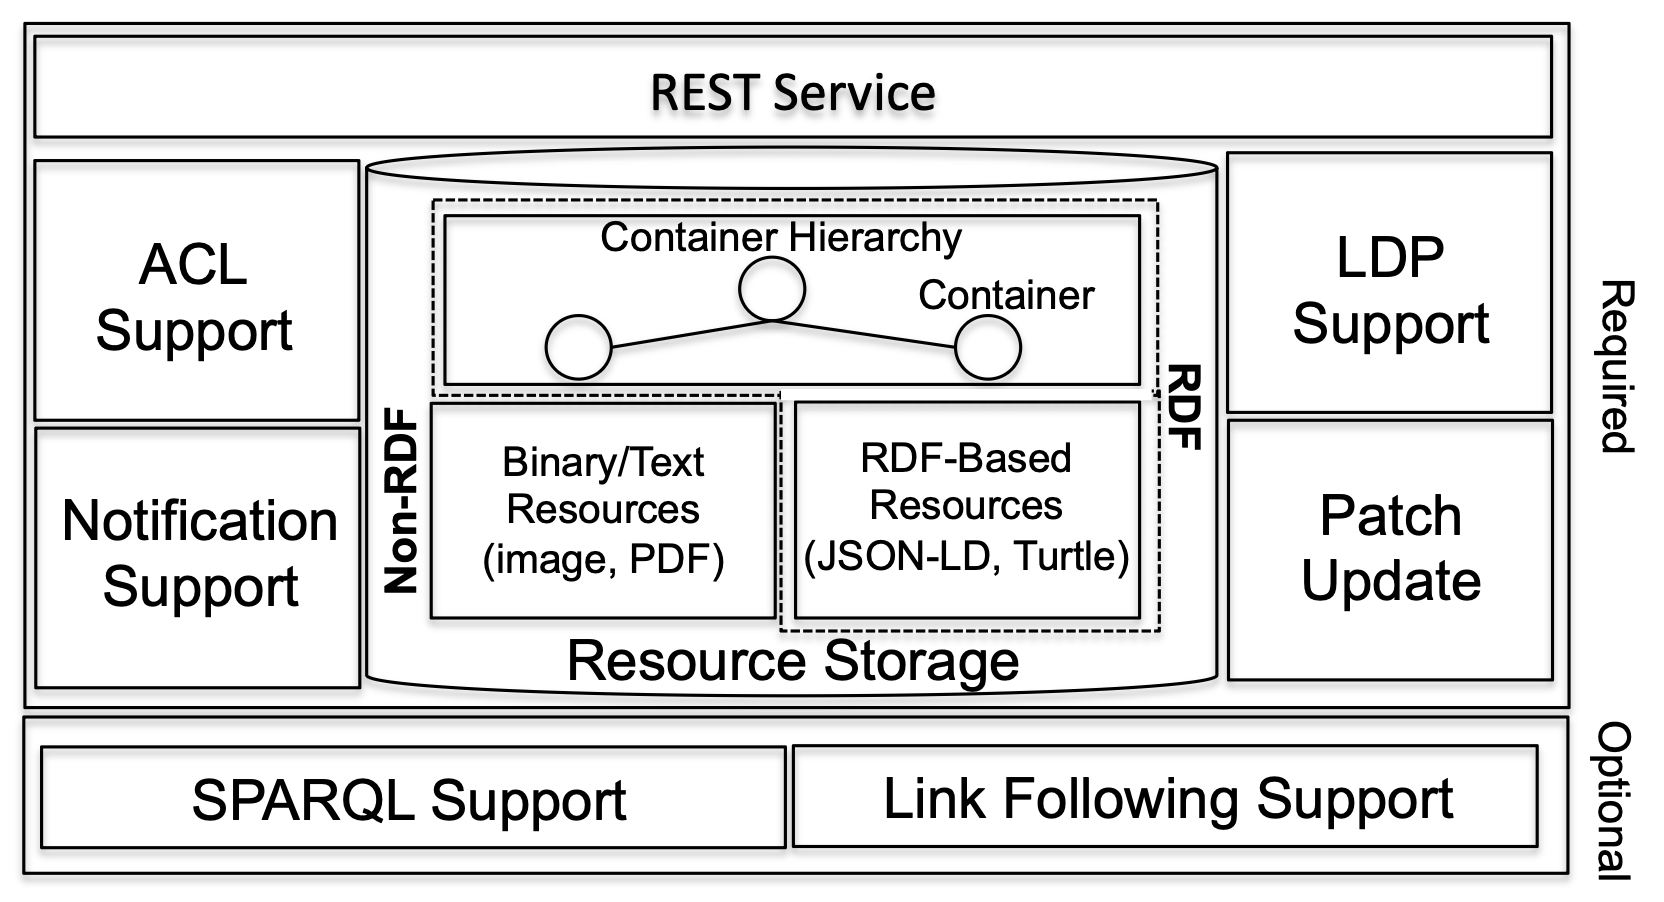
\includegraphics[width=0.8\textwidth]{../shared/assets/sambra_pod_architecture.png}
    \caption{Pod"=Architektur~\cite{sambraSolidPlatformDecentralized2016}}
\end{figure}

\begin{itemize}
    \item Verwendung von LDP für Organisation von Daten in Containern zur Gruppierung von Ressourcen~\cite{sambraSolidPlatformDecentralized2016}
    
    \item Speichern von Ressourcen
    \begin{itemize}
        \item mehrere Möglichkeiten: bspw. Dateisystem, Key"=Value"=Store, relationale Datenbank, Graph"=Datenbanksystem (bspw. RDF"=Store)~\cite{sambraSolidPlatformDecentralized2016}
        \item RDF"=DB vereinfacht große Queries und CRUD, aber Unterstützung von LDP und ACL aufwendiger als bei Dateisystem~\cite{sambraSolidPlatformDecentralized2016}
    \end{itemize}
    
    \item \emph{Resource Patching}
    \begin{itemize}
        \item grundlegende LDP"=Operationen: \texttt{GET}, \texttt{POST}, \texttt{DELETE} und \texttt{HEAD}~\cite{sambraSolidPlatformDecentralized2016}
        \item ggf. spezielle Adapter notwendig je nach Art der Ressource und Ressourcenspeicher
        \item grundlegende SPARQL"=Queries für Patch von Ressourcen (\texttt{DELETE}, \texttt{INSERT})~\cite{sambraSolidPlatformDecentralized2016}
    \end{itemize}

    \item Access Control
    \begin{itemize}
        \item Anwendung kann ggf. nicht nur auf eigene, sondern auch auf Pods anderer User zugreifen~\cite{sambraSolidPlatformDecentralized2016}
        \item verschiedene Zugriffe auf Ressourcen je nach Agent möglich~\cite{sambraSolidPlatformDecentralized2016}
        \item Verwendung der \emph{WebAccessControl} (WAC) Ontologie~\cite{sambraSolidPlatformDecentralized2016}
        \begin{itemize}
            \item Zugriffskontrolle auf Ebene von Containern / Ressourcen~\cite{sambraSolidPlatformDecentralized2016}
            \item Read, Write, Control und Append~\cite{sambraSolidPlatformDecentralized2016}
        \end{itemize}
        \item Realisierung über ACL"=Ressource~\cite{sambraSolidPlatformDecentralized2016}
        \item Ressource kann eigene ACL"=R. haben (\texttt{ressource.acl}), sonst Erben vom Eltern"=Container (\texttt{.acl})~\cite{sambraSolidPlatformDecentralized2016}
        \item Advertisement der URI der ACL"=R. via Link"=Header
    \end{itemize}

    \item Live Updates / Notification Support
    \begin{itemize}
        \item Live Updates bei Modifikation einer Ressource~\cite{sambraSolidPlatformDecentralized2016}
        \item Umsetzung via WebSocket"=Protokoll, PubSub"=System~\cite{sambraSolidPlatformDecentralized2016}
        \begin{itemize}
            \item \verb|sub https://example.org/data/ressource|
            \item \verb|pub https://example.org/data/ressource|
        \end{itemize}
    \end{itemize}

    \item optional SPARQL"=Support (s.o.)~\cite{sambraSolidPlatformDecentralized2016}
\end{itemize}


\subsection{Solid-Anwendungen}
\hl{TODO: andere Überschrift}

\begin{itemize}
    \item Garantie von effizienter Performance durch Solid"=Protokolle~\cite{sambraSolidPlatformDecentralized2016}
    \item beschleunigte Anwendungsentwicklung durch Auslagerung von Standardfunktionalitäten~\cite{sambraSolidPlatformDecentralized2016}
    
    \item Verwendung von Solid"=Anwendungen~\cite{sambraSolidPlatformDecentralized2016}
    \begin{itemize}
        \item Registrierung bei Pod Provider
        \item Abruf einer WebID + Data Storage
        \item Anwendungen speichern Daten im Nutzer-Pod, Zugriff via LDP
    \end{itemize}

    \item Speicherung von Daten in Pod, Wahl einer sinnvollen Container"=Hierarchie sowie Granularität~\cite{sambraSolidPlatformDecentralized2016}

    \item Solid"=Anwendung kann auf Ressourcen anderer Solid"=Anwendungen zugreifen~\cite{sambraSolidPlatformDecentralized2016}
    \begin{itemize}
        \item Kontrolle über ACL~\cite{sambraSolidPlatformDecentralized2016}
        \item[$\Rightarrow$] Interoperabilität auf Daten"=Ebene (statt Anwendungsebene)~\cite{sambraSolidPlatformDecentralized2016}
        \item[$\Rightarrow$] einfacher Wechsel zwischen Anwendungen möglich~\cite{sambraSolidPlatformDecentralized2016}
    \end{itemize}

    \item Unterstützung innovativer sozialer Funktionen, Finden und Teilen von Ressourcen basierend auf \emph{Social Graph}~\cite{sambraSolidPlatformDecentralized2016}
\end{itemize}


\subsection{Erweiterung: B2B-Datenwertschöpfungsketten}

\textbf{Motivation}~\cite{bothSolidBasedB2BData2025}
\begin{itemize}
    \item automatisierte Datenübertragung essenziell für Partner in einer Wertschöpfungskette
    \item verschiedene Anforderungen zur Ausnutzung von daten"=getriebenen Services
    \begin{itemize}
        \item Maschinen"=Lesbarkeit des gesamten Datenaustauschs $\Rightarrow$ automatisierbar
        \item Erfüllung rechtlicher Rahmenbedingungen: weitere Metadaten notwendig, bspw. Zweck für Data Sharing
        \item Nachvollziehbarkeit, Robustheit
    \end{itemize}
    \item Solid bildet bereits Grundlage, aber noch nicht ausreichend
    \item Teilen und Verknüpfen von Daten in B2B"=Umgebungen ohne \emph{alle} Daten zu teilen oder Informationen über Geschäftspartner preiszugeben
    \begin{itemize}
        \item Technologie zum Datenaustausch bei Bedarf
        \item Möglichkeit von \emph{Constraints} beim Data Sharing
    \end{itemize}
    \item Erweiterung des Prozesses, V: universal unterstützte E2E"=Daten"=Wertschöpfungskette
\end{itemize}

\vspace{1cm}

\textbf{Umsetzung der Anforderungen}~\cite{bothSolidBasedB2BData2025}
\begin{itemize}
    \item Maschinen"=Lesbarkeit
    \begin{itemize}
        \item zusätzliche Metadaten: Angabe eines \emph{Data Processing Purpose}s $P$
        \begin{itemize}
            \item repräsentiert minimal mögliche und notwendige Rechte
        \end{itemize}
        \item Weitergabe von Daten unter mind. genauso starken Restriktionen
        \item in Metadaten wird zu einer Purpose"=Klasse verlinkt, welche entlang der Kette weitergegeben wird
    \end{itemize}
    
    \item Weitergabe muss ursprüngliche Quelle verstecken, aber angeben, dass und wie es weitergegeben wurde $\to$ Nachvollziehbarkeit (bspw. externe Audits)
    \begin{itemize}
        \item Erweiterung der Metadaten
        \item Anzeigen, dass Zugriffsrechte und Daten auf Freigabe durch Drittpartei basieren
        \item Einführung einer \emph{Facade}-Klasse zum Verstecken des ursprüngliche Data Providers
    \end{itemize}
\end{itemize}

\vspace{1cm}

\textbf{Fazit}~\cite{bothSolidBasedB2BData2025}
\begin{itemize}
    \item weiterer Schritt in Richtung E2E-Verarbeitung von B2B Data Sharing und Weitergabe unter Berücksichtigung von Datensouveränität
    \item Repräsentation über Linked Data $\to$ vollständig automatisierbare Verarbeitung + Nachvollziehbarkeit + Schutz von Geschäftsgeheimnissen
\end{itemize}


\subsection{Verwandte Konzepte}
